
\documentclass[a4paper]{article}

%Пакеты для математических символов:
\usepackage{amsmath} % американское математическое сообщество.
\usepackage{amssymb} % миллион разных значков и готический, ажурный шрифты.
\usepackage{amscd} % диаграммы, графики.
\usepackage{amsthm} % окружения теорем, определений и тд.
\usepackage{physics} % основные физические символы
%\usepackage{latexsym} % треугольники и пьяная стрелка.

%пакеты для шрифтов:
%\usepackage{euscript} % прописной шрифт с завитушками.
\usepackage{MnSymbol} % Значеки доказательства
\usepackage{verbatim} % улучшенный шрифт "пишущей машинки".
%\usepackage{array} % более удобные таблицы.
%\usepackage{multirow} % мультистолбцы в таблицах.
%\usepackage{longtable} % таблицы на несколько страниц.
%\usepackage{latexsym}

\usepackage{etoolbox}
\usepackage{slashbox} %Разделениени текста \backslashbox{}{}
\usepackage{collectbox} % Добавляет коробочки, можно складывать туда текст)


\usepackage{hyperref} % Ссылки как внешние так и внутренние
\hypersetup{
    colorlinks=true,
    linkcolor=black,
    filecolor=magenta,      
    urlcolor=cyan,
    pdftitle={Overleaf Example},
    pdfpagemode=FullScreen,
    }
    
%Пакеты для оформления:
\RequirePackage[center, medium]{titlesec}% Стиль секций и заголовков
%\usepackage[x11names]{xcolor} % 317 новых цветов для текста.
\usepackage{float} % Позволяет использовать H, h! для локации фигур
%\usepackage{multicol} % набор текста в несколько колонн.
\usepackage{graphicx} % расширенные возможности вставки стандартных картинок.
\usepackage{subcaption} % возможность вставлять картинки в строчку
%\usepackage{caption} % возможность подавить нумерацию у caption.
\usepackage{wrapfig} % вставка картинок и таблиц, обтекаемых текстом.
\usepackage{cancel} % значки для сокращения дробей, упрощения, стремления.
\usepackage{misccorr} % в заголовках появляется точка, но при ссылке на них ее нет.
%\usepackage{indentfirst} % отступ у первой строки раздела
%\usepackage{showkeys} % показывает label формул над их номером.
%\usepackage{fancyhdr} % удобное создание верхних и нижних колонтитулов.
%\usepackage{titlesec} % еще одно создание верхних и нижних колонтитулов
\usepackage{hyperref} % Ссылки как внешние так и внутренние
\hypersetup{
    colorlinks=true,
    linkcolor=black,
    filecolor=magenta,      
    urlcolor=cyan,
    pdftitle={Overleaf Example},
    pdfpagemode=FullScreen,
    }
\usepackage{xcolor} %Позволяет перекрасить все страници
\definecolor{mycolor}{RGB}{244,228,215} %Цвет перекраски


%Пакеты шрифтов, кодировок. НЕ МЕНЯТЬ РАСПОЛОЖЕНИЕ.
\usepackage[utf8]{inputenc} % кодировка символов.
%\usepackage{mathtext} % позволяет использовать русские буквы в формулах. НЕСОВМЕСТИМО С tempora.
\usepackage[T1, T2A]{fontenc} % кодировка шрифта.
\usepackage[english, russian]{babel} % доступные языки.


%Отступы и поля:
%размеры страницы А4 11.7x8.3in
\textwidth=7.3in % ширина текста
\textheight=10in % высота текста
\oddsidemargin=-0.5in % левый отступ(базовый 1дюйм + значение)
\topmargin=-0.5in % отступ сверху до колонтитула(базовый 1дюйм + значение)


%Сокращения
%Скобочки
\newcommand{\inrad}[1]{\left( #1 \right)}
\newcommand{\inner}[1]{\left( #1 \right)}
\newcommand{\infig}[1]{\left{ #1 \right}}
\newcommand{\insqr}[1]{\left[ #1 \right]}
\newcommand{\ave}[1]{\left\langle #1 \right\rangle}



%% Красивые <= и >=
\renewcommand{\geq}{\geqslant}
\renewcommand{\leq}{\leqslant}

%%Значек выполнятся
\newcommand{\per}{\hookrightarrow}

%%Векторная алгебра
\newcommand{\rot}{\text{rot}}
\renewcommand{\div}{\text{div}}
\renewcommand{\grad}{\text{grad}}

%% Более привычные греческие буквы
\renewcommand{\phi}{\varphi}
\renewcommand{\epsilon}{\varepsilon}
\newcommand{\eps}{\varepsilon}
\newcommand{\com}{\mathbb{C}}
\newcommand{\re}{\mathbb{R}}
\newcommand{\nat}{\mathbb{N}}
\newcommand{\stp}{$\filledmedtriangleleft$}
\newcommand{\enp}{$\filledmedsquare$}

%%Тензорный анализ ОТО теория поля
\newcommand{\Li}[1]{\mathfrak{L}_{#1}}
\newcommand{\crist}[3]{\cfrac{1}{2} \inner{g_{#1#2,#3} + g_{#1#3,#2} - g_{#2#3,#1}}}
\newcommand{\piv}[2]{\cfrac{\partial #1}{\partial #2}}

\makeatletter
\newcommand{\sqbox}{%
    \collectbox{%
        \@tempdima=\dimexpr\width-\totalheight\relax
        \ifdim\@tempdima<\z@
            \fbox{\hbox{\hspace{-.5\@tempdima}\BOXCONTENT\hspace{-.5\@tempdima}}}%
        \else
            \ht\collectedbox=\dimexpr\ht\collectedbox+.5\@tempdima\relax
            \dp\collectedbox=\dimexpr\dp\collectedbox+.5\@tempdima\relax
            \fbox{\BOXCONTENT}%
        \fi
    }%
}
\makeatother
\newcommand{\mergelines}[2]{
\begin{tabular}{llp{.5\textwidth}}
#1 \\ #2
\end{tabular}
}
\newcommand\tab[1][0.51cm]{\hspace*{#1}}
\newcommand\difh[2]{\frac{\partial #1}{\partial #2}}
\newcommand{\messageforpeople}[1]{HSE Faculty of Physics \ \ HSE Faculty of Physics HSE Faculty of Physics \ \ HSE Faculty of Physics HSE Faculty of Physics \ \ HSE Faculty of Physics HSE Faculty of Physics \ \ HSE Faculty of Physics HSE Faculty of Physics \ \ HSE Faculty of Physics HSE Faculty of Physics \ \ HSE Faculty of Physics HSE Faculty of Physics \ \ HSE Faculty of Physics HSE Faculty of Physics \ \ HSE Faculty of Physics }


\numberwithin{equation}{section}

\begin{document}


\begin{flushright}
    Выполнил:
    Карибджанов Матвей

    Домашняя работа № 6
\end{flushright}
\newpagestyle{main}{
\setfootrule{0.4pt}
\setfoot{}{\thepage}{Домашняя работа \ № \ 6}}
\pagestyle{main}
% \pagecolor{mycolor}

Задание найти прцессию спина электрона. Пусть электрон вращается с поcтоянной 
угловой скростью вокруг ядра, тогда можем выразить 4-скрость и 4-ускорение так.


\begin{gather}
    x = 
    \begin{pmatrix}
        t \\ r\cos(\omega t) \\ r\sin(\omega t) \\ 0
    \end{pmatrix}
\end{gather}

\begin{gather}
    u = 
    \gamma
    \begin{pmatrix}
        1 \\ -r\omega\sin(\omega t) \\ r\omega\cos(\omega t) \\ 0
    \end{pmatrix}
\end{gather}

\begin{gather}
    w =  -\gamma^2 \omega^2 r
    \begin{pmatrix}
        0 \\ \cos(\omega t) \\ \sin(\omega t) \\ 0
    \end{pmatrix}
\end{gather}

Для решения воспользекмся производной Ферми-Уокера, котрая занутся в для
системы свободных гироскопов.

\begin{eqnarray}
    \piv{A^i}{s} - \Gamma_{jk}^{i} u^j A^k + \inner{u_iw_j - u_jw_i}A^i = 0
\end{eqnarray}

Так как работаем в инерциальной системе отсчета, то $\Gamma = 0$. Так же 
в ситеме отчета чатици, спин обладает только координатными компонентам, а 
4-скорост частици будет иметь только всеменную компонету, тогда получим 
что $u_iA^i =0$.

\begin{eqnarray}
    \piv{A^i}{s} - u_jw_iA^i = 0
\end{eqnarray}

\begin{gather}
    \begin{pmatrix}
        \gamma\piv{A^0}{t} \\ \gamma\piv{A^1}{t} \\ \gamma\piv{A^2}{t} \\ \gamma\piv{A^3}{t}
    \end{pmatrix}
    =
    -\gamma^3 \omega r \inner{\cos{\omega t}A^1 + \sin{\omega t}A^2}
    \begin{pmatrix}
        1 \\ -\omega r\sin(\omega t) \\ \omega r\cos(\omega t) \\ 0
    \end{pmatrix}
\end{gather}

\begin{figure}[H]
    \centering
    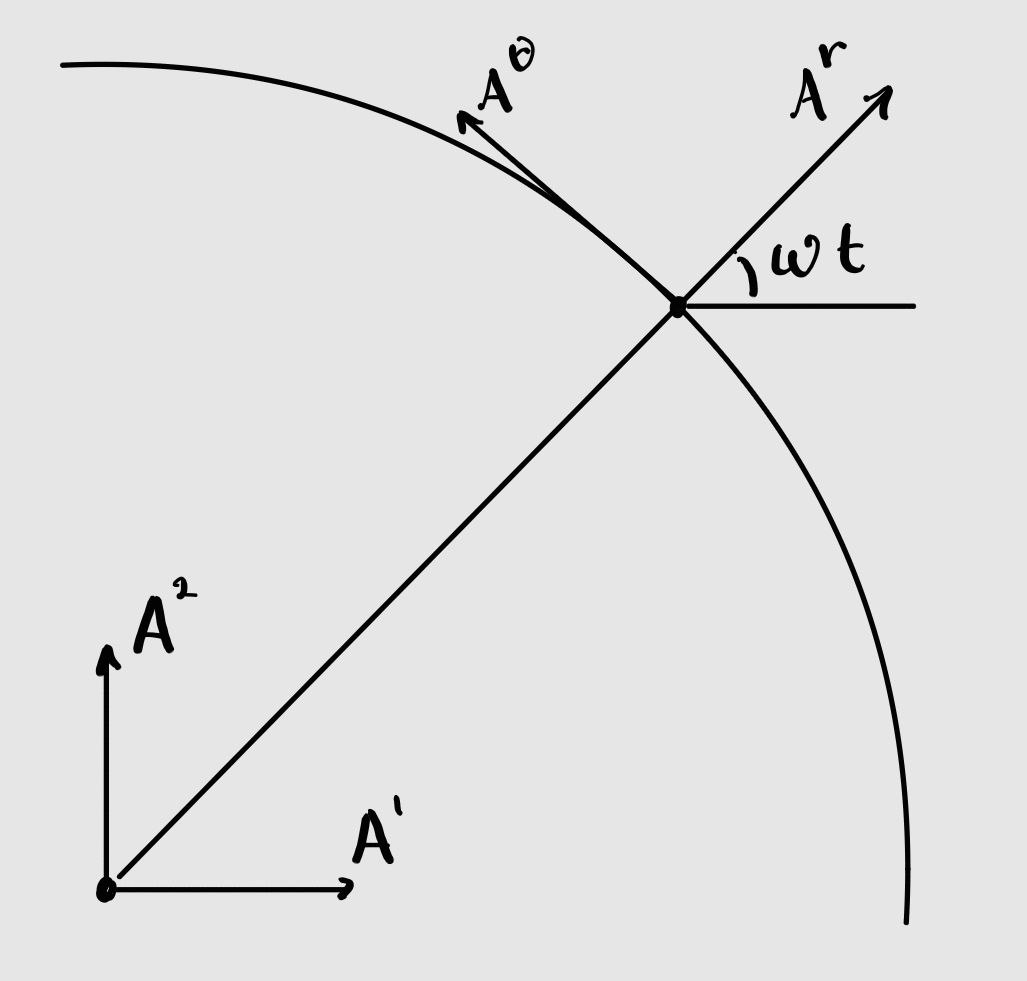
\includegraphics[width=0.4\textwidth]{sp.jpg}
\end{figure}

\begin{eqnarray}
    A^1 = A^r \cos{\omega t} - A^\theta \sin{\omega t} \\
    A^2 = A^r \sin{\omega t} + A^\theta \cos{\omega t} \\
\end{eqnarray}

\begin{eqnarray}
    A^r = A^1 \cos{\omega t} + A^2 \sin{\omega t} \\
    A^\theta = -A^1 \sin{\omega t} + A^2 \cos{\omega t} \\
\end{eqnarray}


\begin{eqnarray}
    \piv{A^r}{t} = \omega A^\theta \\
    \piv{A^\theta}{t} = -\omega \gamma^2 A^r
\end{eqnarray}

\begin{gather}
    \begin{pmatrix}
        \cfrac{d A^r}{d t} \\
        \cfrac{d A^\theta}{d t}  
    \end{pmatrix}
    = 
    \begin{pmatrix}
        0 & \omega\\
        -\gamma^2 \omega & 0
    \end{pmatrix}
    \begin{pmatrix}
        A^r \\ A^\theta
    \end{pmatrix}
\end{gather}

\begin{gather}
    \lambda_1 = i \gamma \omega, \ 
    h_1 =
    \begin{pmatrix}
        -i/\gamma \\ 1
    \end{pmatrix}; \
    \lambda_2 = -i \gamma \omega, \ 
    h_2 =
    \begin{pmatrix}
        i/\gamma \\ 1
    \end{pmatrix}, \
\end{gather}

\begin{gather}
    \begin{pmatrix}
        A^r \\ A^\theta
    \end{pmatrix}
    =
    C_1 
    \begin{pmatrix}
        -i/\gamma \\ 1
    \end{pmatrix}
    \exp\inner{i\gamma \omega t}
    +
    C_2
    \begin{pmatrix}
        i/\gamma \\ 1
    \end{pmatrix}
    \exp\inner{-i\gamma \omega t}
\end{gather}

\begin{gather}
    \begin{pmatrix}
        A^r \\ A^\theta
    \end{pmatrix}
    =
    C
    \begin{pmatrix}
        \cos \inner{\omega \gamma t + \phi} \\        
        \gamma \sin \inner{\omega \gamma t + \phi}        
    \end{pmatrix}
\end{gather}

\begin{gather}
    A =
    \begin{pmatrix}
        C \insqr{\cos \inner{\omega \gamma t + \phi} \cos \omega t 
        + \gamma \sin  \inner{\omega \gamma t + \phi} \sin \omega t} \\
        C \insqr{\cos \inner{\omega \gamma t + \phi} \sin \omega t -
        \gamma \sin \inner{\omega \gamma t + \phi} \cos \omega t}
    \end{pmatrix}
\end{gather}

В итоге получи приращение за оборот:

\begin{gather}
    \Delta A = 
    \begin{pmatrix}
        C \insqr{\cos \phi - \cos(2\pi\gamma + \phi)}\\
        - C \gamma \insqr{\sin \phi - \sin(2\pi\gamma + \phi)}
    \end{pmatrix}
\end{gather}

\end{document}